% DO NOT COMPILE THIS FILE DIRECTLY!
% This is included by the other .tex files.

\begin{frame}[t,plain]
\titlepage
\end{frame}

\begin{frame}
	\frametitle{Plan for this session}
	\begin{itemize}
		\item Quick introduction of what MISP is
                \item How can ISACs use MISP?
                \item Working with unique use-cases
	\end{itemize}
\end{frame}

\begin{frame}
 \frametitle{MISP and starting from a practical use-case}
 \begin{itemize}
         \item During a malware analysis workgroup in 2012, we discovered that we worked on the analysis of the same malware.
         \item We wanted to share information in an easy and automated way {\bf to avoid duplication of work}.
         \item Christophe Vandeplas (then working at the CERT for the Belgian MoD) showed us his work on a platform that later became MISP.
         \item A first version of the MISP Platform was used by the MALWG and {\bf the increasing feedback of users} helped us to build an improved platform.
         \item MISP is now {\bf a community-driven effort}.
 \end{itemize}
\end{frame}

\begin{frame}
\frametitle{Development based on practical user feedback}
\begin{itemize}
\item There are many different types of users of an information sharing platform like MISP:
        \begin{itemize}
                \item {\bf Malware reversers} willing to share indicators of analysis with respective colleagues.
                \item {\bf Security analysts} searching, validating and using indicators in operational security.
                \item {\bf Intelligence analysts} gathering information about specific adversary groups.
                \item {\bf Law-enforcement} relying on indicators to support or bootstrap their DFIR cases.
                \item {\bf Risk analysis teams} willing to know about the new threats, likelyhood and occurences.
                \item {\bf Fraud analysts} willing to share financial indicators to detect financial frauds.
        \end{itemize}
\end{itemize}
\end{frame}

\begin{frame}
 \frametitle{So, what is MISP nowadays?}
 \begin{itemize}
         \item MISP\footnote{\url{https://github.com/MISP/MISP}} is a threat information sharing platform that is free \& open source.
         \item MISP has {\bf a host of functionalities} that assist users in creating, collaborating \& sharing threat information.
         \item Long list of connectors to support most of the tooling used by security teams (IDS, Siems, host sensors, analysis tools, etc).
         \item A rich set of MISP modules\footnote{\url{https://www.github.com/MISP/misp-modules}} to connect to a wide range of services, easily extended by the users.
         \item Tools to manage sharing communities and interconnected MISP servers
 \end{itemize}
\end{frame}

\begin{frame}
\frametitle{MISP distributed sharing functionality}
\begin{itemize}
\item MISPs' core functionality is sharing where everyone can be a {\bf consumer and/or a contributor/producer}."
\item Quick benefit without the obligation to contribute.
\item {\bf Low barrier of entry} to get acquainted with the system.
\end{itemize}
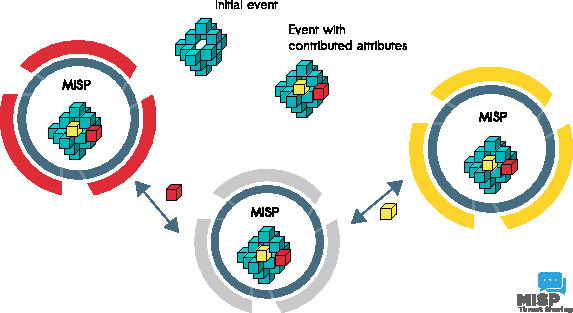
\includegraphics[scale=0.9]{misp-distributed.pdf}
\end{frame}

\begin{frame}
\frametitle{Information quality management}
    \begin{itemize}
        \item Correlating data
        \item Feedback loop from detections via {\bf Sightings}
        \item {\bf False positive management} via the warninglist system
        \item {\bf Enrichment system} via MISP-modules
        \item {\bf Integrations} with a plethora of tools and formats
        \item Flexible {\bf API} and support {\bf libraries} such as PyMISP to ease integration
        \item {\bf Timelines} and giving information a temporal context
        \item Full chain for {\bf indicator life-cycle management}
    \end{itemize}
\end{frame}

\begin{frame}
        \frametitle{Correlation features: a tool for analysts}
        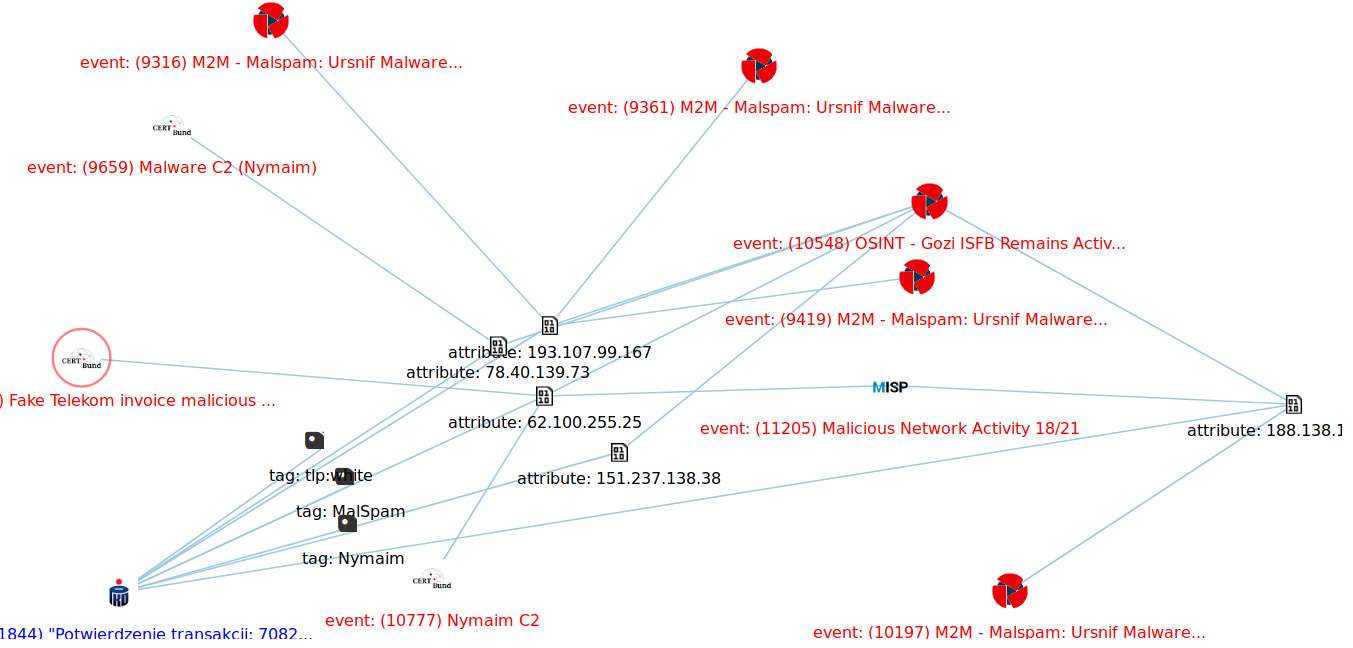
\includegraphics[scale=0.18]{campaign.png}
        \begin{itemize}
                \item To {\bf corroborate a finding} (e.g. is this the same campaign?), {\bf reinforce an analysis} (e.g. do other analysts have the same hypothesis?), {\bf confirm a specific aspect} (e.g. are the sinkhole IP addresses used for one campaign?) or just find if this {\bf threat is new or unknown in your community}.
        \end{itemize}
\end{frame}


\begin{frame}
\frametitle{What sort of sharing scenarios make sense for ISACs?}
    \begin{itemize}
        \item Exchange of {\bf insights from monitoring}
        \item Sharing the outcomes of {\bf incidents} (often technical only)
        \item Information on the {\bf attackers, techniques used}
        \item {\bf Remediation} information / {\bf prevention} information
        \item {\bf Vulnerability} pre-disclosure
        \item Supporting {\bf tools / scripts}
    \end{itemize}
\end{frame}

\begin{frame}
\frametitle{Other types of exchanges we've seen (often by sectorial ISACs)}
    \begin{itemize}
        \item {\bf Financial fraud} information sharing
        \item Law enforcement / Border control specific sharing
        \item {\bf Disinformation} sharing
        \item {\bf Health} related information sharing
    \end{itemize}
\end{frame}

\begin{frame}
 \frametitle{An example of an alternate use-case: COVID-19 MISP}
 \begin{itemize}
         \item COVID-19 MISP is a MISP instance retrofitted for COVID-19 info sharing
         \item We are focusing on three areas of sharing:
         \begin{itemize}
              \item {\bf Medical} information
              \item {\bf Cyber threats} related to / abusing COVID-19
              \item {\bf Disinformation} campaigns abusing COVID-19
         \end{itemize}
         \item Low barrier of entry, aiming for wide spread
         \item Already a {\bf massive community}
 \end{itemize}
\end{frame}

\begin{frame}
    \frametitle{COVID-19 MISP dashboard (medical data part)}
    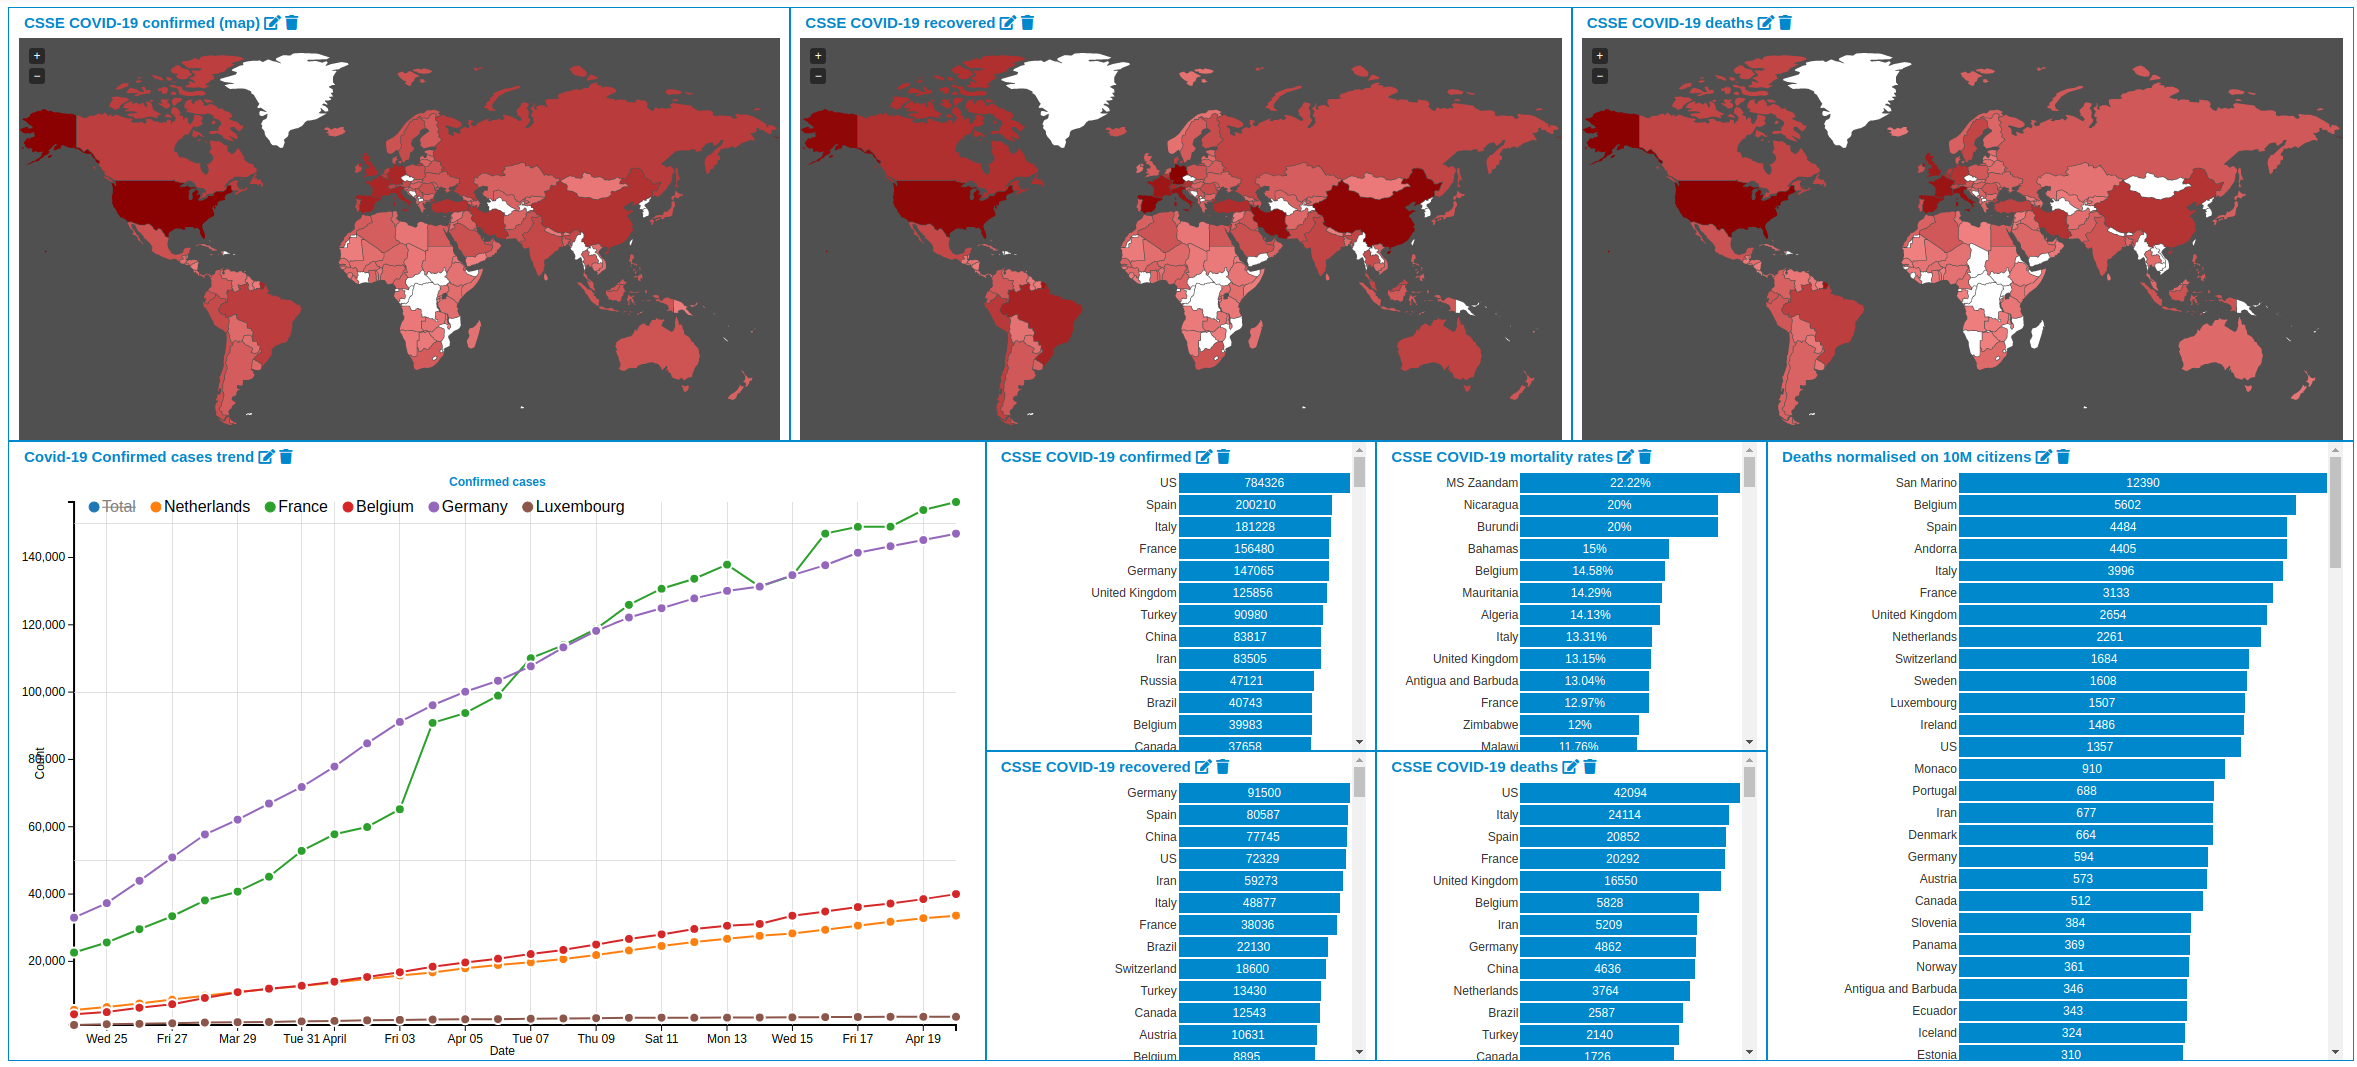
\includegraphics[width=1.00\linewidth]{dashboard.png}
    We are rapidly building new models for the different COVID-19 related information sources
\end{frame}

\begin{frame}
\frametitle{Getting started with communities for ISACs}
\begin{itemize}
	\item Different models for constituents
	\begin{itemize}
        \item {\bf Connecting to} a MISP central instance hosted by the ISAC
        \item {\bf Hosting} their own instance and connecting to CSIRT's MISP
        \item The ISAC member becoming a "{\bf hub}" for a connected (sub-) community 
	\end{itemize}
	\item Additional services potentially offered
	\begin{itemize}
		\item Access to {\bf shared services / subscriptions}
		\item Offering {\bf services} directly through MISP (assisting in incident resolution, etc)
		\item {\bf Collaboration} between members
	\end{itemize}
\end{itemize}
\end{frame}

\begin{frame}
\frametitle{The arsenal to make it all happen}
\begin{itemize}
	\item ISAC specific {\bf common vocabularies}
        \item Common tooling / integration options
	\begin{itemize}
        \item Already existing, self-built or simply reach out to us for support
        \end{itemize}
        \item Community management tooling
        \item {\bf Massive adoption} of MISP means a lot of your members probably already know the tool
\end{itemize}
\end{frame}

\begin{frame}
\frametitle{What do members of a community get out of all of this?}
    \begin{itemize}
        \item {\bf Herd immunity} through automatable, actionable protection/detection
        \item A {\bf collaboration} platform
        \item Derived metrics and situational awareness to identify gaps / focus areas
        \item Making {\bf canonisation} and {\bf conversion} of their data sources straight forward for their tooling
        \item {\bf Near real-time exchange} of automated information
    \end{itemize}
\end{frame}

\begin{frame}
\frametitle{So what's the next step once your sharing community is thriving?}
\begin{itemize}
	\item Getting your community to be active takes {\bf time and effort}, but with persistence your chances are great.
	\item However, most of these communities end up being in a {\bf sectorial/geographic silo}
	\item The next step is to become part of a network of ISACs, {\bf join broader sharing communities}
\end{itemize}
\end{frame}

\begin{frame}
\frametitle{Advantages of cross sectorial sharing}
\begin{itemize}
	\item {\bf Reuse of TTPs} across sectors
	\item Being hit by something that {\bf another sector has faced before}
	\item {\bf Hybrid threats} - how seemingly unrelated things may be interesting to correlate
	\item Prepare other communities for the capability and {\bf culture of sharing} for when the need arises for them to reach out to CSIRT
	\item Generally our field is ahead of several other sectors when it comes to information sharing, might as well {\bf spread the love}
\end{itemize}
\end{frame}


\begin{frame}
        \frametitle{Conclusion}
        \begin{itemize}
                \item MISP is just a tool. What matters is your sharing practices. The tool should be as transparent as possible to support you.
                \item Enable users to customize MISP to meet their community's use-cases.
                \item MISP project combines open source software, open standards, best practices and communities to make information sharing a reality.
        \end{itemize}
\end{frame}

\begin{frame}
\frametitle{Get in touch if you need some help to get started}
\begin{itemize}
\item Getting started with building a new community can be daunting. Feel free to get in touch with us if you have any questions!
\item Contact: info@circl.lu
\item \url{https://www.circl.lu/}
\item \url{https://github.com/MISP}  \url{https://gitter.im/MISP/MISP}  \url{https://twitter.com/MISPProject}
\end{itemize}
\end{frame}

